%!TEX root = ../MasterThesis.tex

\section{The Semantic Web}
\label{sec:semantic_web}

The \emph{Semantic Web} initiative strives for a better integration of distributed data from various publishers on the Web to enable new kinds of Smart Web applications. To achieve this goal, the Semantic Web delivers the infrastructure for this vision in form of various standard specifications such as \gls{RDF}, \gls{RDFS}, \gls{OWL}, \gls{SPARQL}, \ldots, which are introduced during the course of this section. Before going into the technical specifications of these the section shows the fundamental aspects underlying the (Semantic) Web as a whole.

\subsection{Fundamental aspects}
\label{subsec:fundamentals_semweb}

The Semantic Web builds on the fundamentals of the existing World-Wide Web, especially \citep[pg. 4-11]{allemang2011semantic}: \@

\begin{itemize}
	\item \textbf{AAA-Slogan:} Anyone can say Anything about Any topic. The Web does not restrict what people can post or publish on it. It is in the responsibilities of the readers to decide whether they can trust information from a specific source or not.
	\item \textbf{Open World Assumption:} as the amount of information on the Web is endless, and new information is published every day, one must always assume that there are new information available on it, that one does not know yet. As of this one can never be sure to have all facts at hand. New information can be published at any time that can give additional insights.
	\item \textbf{Non-unique Naming Assumption:} there is no central authority, who is responsible for providing unique identifiers for entities on the Web. Due to this fact different \gls{URI}s might refer to the same entity or real-world object.
\end{itemize}

Instead of making information on the Web available for human consumption \emph{only}, the Semantic Web is trying to make the information on the Web accessible (and readable) to machines as well. This will allow the integration of information across Web sites, and enable a distributed, interlinked ``Web of Data''. The major design principles to achieve this objective are \citep[pg. 1-22]{antoniou2008semantic}: \@

\begin{enumerate}
	\item make structured and semi-structured data available in standard formats,
	\item make individual data elements and their relationships accessible on the Web,
	\item describe the intended semantics of the data in a machine readable format
\end{enumerate}

The data model of the Semantic Web is build upon labeled graphs with objects and their relationships. Objects are modeled as nodes and their relationships as edges between them. To express these graphs of objects and their relationships, the Semantic Web: \@

\begin{itemize}
	\item formalize the syntax of the graph in \gls{RDF} (see Section~\ref{sec:semantic_rdf}),
	\item use \gls{URI}s to identify individual data items and relations (see Section~\ref{subsec:uri_concept}),
	\item use ontologies to represent semantics of the entities. Ontologies can be lightweight \gls{RDFS} definitions or expressive descriptions in the \gls{OWL} language (see Section~\ref{sec:semantic_vocab_ontologies}).
\end{itemize}

Initially it was tried to solve the data integration aspect on the Web with the exchange of \gls{XML} based messages, but though the \gls{XML} format is more machine-readable as \gls{HTML} it still lacks the semantic of the data transmitted (see Section~\ref{subsec:xml_format}). Therefore the Semantic Web defines the \gls{RDF} format as the basic data exchange format of it. Still the \gls{RDF} format was initially based on the \gls{XML} specification. To formally describe the existing terms and their relationships within a domain the Semantic Web relies on an ontology specification. These specifications are either expressed in \gls{RDFS} or uses the more expressive \gls{OWL} language; both of them are meta-description languages, which allows the definition of domain-specific knowledge representations based on the concepts found in \gls{RDF} itself. \\

As such the Semantic Web is a layered approach as depicted in Figure~\ref{fig:images_semweb_model}.\@

\begin{figure}[H]
	\centering
		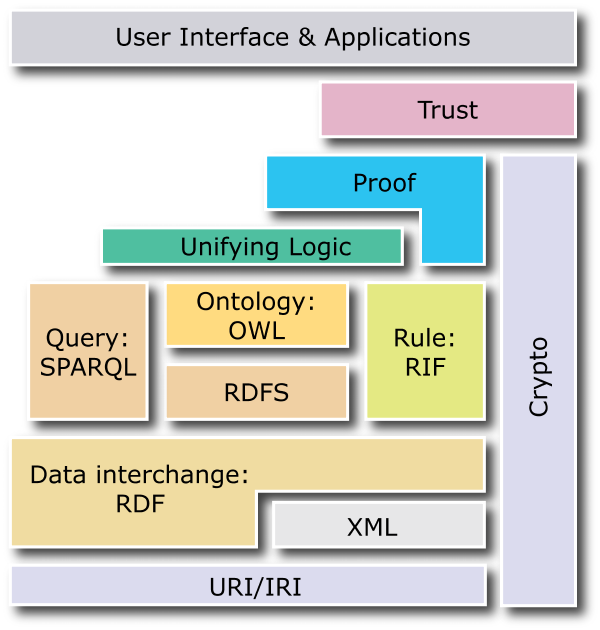
\includegraphics[width=0.8\columnwidth]{images/semantic_web_layers.png}
	\caption[The Semantic Web Model]{The Semantic Web Model \citep{W3C2013}}
\label{fig:images_semweb_model}
\end{figure}

% section semantic_fundamentals (end)

\subsection{A Resource Description Framework}
\label{sec:semantic_rdf}

When trying to come up with a specification on how to integrate data on a globally dispersed platform such as the World-Wide Web, one will have to answer the following questions first: \@

\begin{itemize}
	\item \textbf{syntax:} How to serialize the data?
	\item \textbf{data model:} How to structure and organize the data?
	\item \textbf{semantics:} How to interpret the data?
\end{itemize}

Whereas the World-Wide Web is made up from interlinked documents in the \gls{HTML} format that is specifically designed for rendering information on screen to be consumed by a human, the \gls{RDF} brings a highly flexible data model to the Web. Its basic building block is the \emph{triple}, that is a statement consisting of an entity, an attribute and a value. The parts of a statement are also known as subject, predicate and object, which make up a directed graph as shown in the example in Figure~\ref{fig:images_semweb_triple}: \@

\begin{figure}[H]
	\centering
		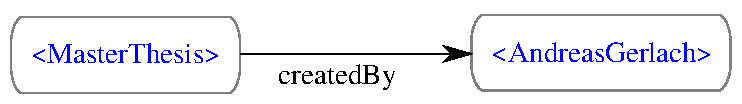
\includegraphics[width=0.8\columnwidth]{images/sample_triple.pdf}
	\caption{A basic example for a triple-statement}
\label{fig:images_semweb_triple}
\end{figure}

In this example the triple consists of the entity ``MasterThesis'', the assigned attribute ``createdBy'' and the value ``AndreasGerlach''. The value-part of a triple can contain either a literal value or another entity (as in the example above). Still a problem with this example statement is that the entities are not unique. Based on the given information it is not clear, which specific ``MasterThesis'' is meant and to whom the value ``AndreasGerlach'' refers. Additionally the predicate shown could have multiple meanings. These ambiguities have to be resolved on the Semantic Web to be able to make these information understandable by machines. To solve these issues the Semantic Web standard specifies that names of entities and predicates have to use a \gls{URI} (see Section~\ref{subsec:uri_concept}) to make their meanings clear. Literals that can be used as values such as numbers, dates and strings borrow their data type specifications from the \gls{XML} standard \citep[pg. 15-38]{wood2014linked}. \\

Based on this description the foundational elements of \gls{RDF} can be summarized as: \@

\begin{itemize}
	\item \textbf{entities:} aka resources or ``things'' of interest that are identified via \gls{URI}s
	\item \textbf{predicates:} aka attributes or properties that specify the relations between resources and are also identified by \gls{URI}s
	\item \textbf{literals:} integral values such as numbers, dates and strings that are based on the \gls{XML} data type specification
	\item \textbf{statements:} assign a value (either another entity or a literal) to a ``entity-predicate'' relation
	\item \textbf{graphs:} as the data model behind \gls{RDF} enables a  distributed, interlinked ``Web of Data''
\end{itemize}

\gls{RDF} triples can be serialized into four different syntax formats \citep[pg. 43-54]{wood2014linked}: \@

\begin{itemize}

	\item \textbf{\gls{RDF}/\gls{XML}:} the original format of the \gls{RDF} specification is based on the \gls{XML} specification. Because of their complexity they are best used with a parser program. For an example see Listing~\ref{lst:xml_meta_data}.
	\item \textbf{\gls{RDFa}:} describes how to embed \gls{RDF} information into existing \gls{HTML} documents. It allows Web site authors to enrich their Web pages with semantic information by adding a set of \gls{HTML} attributes to important items of the document. For an example see Listing~\ref{lst:rdfa_meta_data}.
	\item \textbf{\gls{JSON-LD}:} a recent initiative to allow JavaScript developers to use \gls{JSON} documents to express a \gls{RDF} statement, see Listing~\ref{lst:jsonld_meta_data}
	\item \textbf{Turtle:} a human readable serialization format for \gls{RDF} statements. \gls{URI}s can be shortened with a declared prefix, statements have to be finished with `.'. Statements referring to the same entity can be abbreviated via `;', which repeats the subject from the previous statement, or `,', which repeats subject and predicate from it. For an example see Listing~\ref{lst:turtle_meta_data}.
\end{itemize}

\begin{listing}[H]
	\begin{minted}[linenos,
	               numbersep=5pt,
	               breaklines=true,
	               frame=lines,
								 gobble=2]{XML}
		<?xml version="1.0"?>
		<rdf:RDF xmlns:rdfs="http://www.w3.org/2000/01/rdf-schema#"
			xmlns:ex="http://www.example.com/">
		  <rdf:Description rdf:about="http://www.example.com/MasterThesis">
		    <ex:createdBy rdf:resource="http://www.example.com/AndreasGerlach" />
		  </rdf:Description>
		</rdf:RDF>
	\end{minted}
\caption{A triple statement expressed in \gls{RDF}/\gls{XML} format}
\label{lst:xml_meta_data}
\end{listing}

\begin{listing}[H]
	\begin{minted}[linenos,
	               numbersep=5pt,
	               breaklines=true,
	               frame=lines,
								 gobble=2]{HTML}
	  <div about="http://www.example.com/MasterThesis">
	    <span rel="http://www.example.com/createdBy" resource="http://www.example.com/AndreasGerlach">
	  </div>
	\end{minted}
\caption{A triple statement expressed in \gls{RDFa} format}
\label{lst:rdfa_meta_data}
\end{listing}

\begin{listing}[H]
	\begin{minted}[linenos,
	               numbersep=5pt,
	               breaklines=true,
	               frame=lines,
								 gobble=2]{JSON}
  {
   "@context": "http://www.example.com/",
   "@id": "http://www.example.com/MasterThesis",
   "createdBy": "http://www.example.com/AndreasGerlach"
 	}
	\end{minted}
\caption{A triple statement expressed in \gls{JSON-LD} format}
\label{lst:jsonld_meta_data}
\end{listing}

\begin{listing}[H]
	\begin{minted}[linenos,
	               numbersep=5pt,
	               breaklines=true,
	               frame=lines,
								 gobble=2]{TURTLE}
	  @prefix ex:  <http://www.example.com/> .
	  ex:MasterThesis ex:createdBy ex:AndreasGerlach .
	\end{minted}
\caption{A triple statement expressed in Turle format}
\label{lst:turtle_meta_data}
\end{listing}

Coming back to the initial questions that have to be solved for data integration on a larger scale, this section showed how the Semantic Web tries to solve them, such as this: \@

\begin{itemize}
	\item \textbf{syntax:} supports the following formats: Turtle, \gls{RDFa}, \gls{RDF}/\gls{XML} and \gls{JSON-LD},
	\item \textbf{data model:} graph-based data model in \gls{RDF} specification,
	\item \textbf{semantics:} express semantics of the data in \gls{RDFS}. This will be the topic of the next section.
\end{itemize}

% section semantic_rdf (end)

\subsection{\gls{RDF} vocabularies and Web Ontologies}
\label{sec:semantic_vocab_ontologies}

For describing domain specific semantics of the data in a \gls{RDF} data set one can either use the lightweight \gls{RDFS} standard to define available entities and their relationships, or use the more expressive \gls{OWL} specification from the \gls{W3C}. \\

Both specifications are based on the \gls{RDF} data model, and make use of the following predefined \gls{URI}s to specify their meanings, see Table~\ref{tab:w3c_vocab_rdf}: \@

\begin{table}[H]
\centering
\begin{tabular}{p{3cm}llp{4.5cm}}
\hline
\textbf{Name} & \textbf{Prefix} & \textbf{Describes} & \textbf{Namespace URI} \\
\hline
\gls{RDF} & rdf: & Core \gls{RDF} framework & \url{http://www.w3.org/1999/02/22-rdf-syntax-ns\#} \\
\hline
\gls{RDFS} & rdfs: & Define \gls{RDF} vocabularies & \url{http://www.w3.org/2000/01/rdf-schema\#} \\
\hline
Web Ontology Language & owl: & Define ontologies & \url{http://www.w3.org/2002/07/owl\#} \\
\hline
\end{tabular}
\caption[\gls{RDF} vocabularies specified by the \gls{W3C}]{\gls{RDF} vocabularies specified by the \gls{W3C} \citep[pg. 41]{wood2014linked}}
\label{tab:w3c_vocab_rdf}
\end{table}

An important step in the definition of a \gls{RDF} vocabulary or Web ontology is to analyze the domain in question in-depth, and come up with a list of objects and their relations. One can follow this step-by-step guide \citep[pg. 88-94]{antoniou2008semantic}: \@

\begin{enumerate}
	\item Specify the \emph{things} to talk about. These have to be divided in \emph{objects} (aka real entities) and \emph{classes} (aka set of entities). A specific statement containing the predicate ``rdf:type'' assigns individual objects to their classes.
	\item Set up relations available between classes. These can either be relations of type inheritance or composition.
	\item Define properties (aka predicates) and their hierarchical relationships  if available.
	\item Impose restrictions on the kind of properties that can be used on objects. These can include restrictions on the \emph{values} a predicate might take (aka ``range'' restrictions), and restrictions on the possible \emph{subjects} of a predicate (aka ``domain'' restrictions).
\end{enumerate}

\begin{table}[H]
\centering
\begin{tabular}{p{4cm}p{7cm}}
\hline
\textbf{Predicate} & \textbf{Describes} \\
\hline
rdfs:Resource & resources \\
\hline
rdfs:Class & classes \\
\hline
rdfs:Literal & literals \\
\hline
rdfs:Propery & properties \\
\hline
rdf:type	& kind of class \\
\hline
rdfs:subClassOf 	&	inheritance between classes \\
\hline
rdfs:subPropertyOf 	& inheritance between properties \\
\hline
rdfs:domain	&	subject restriction of a property \\
\hline
rdfs:range  & value restriction of a property \\
\hline
\end{tabular}
\caption[\gls{RDFS} predicates to define \gls{RDF} vocabularies]{\gls{RDFS} predicates to define \gls{RDF} vocabularies \citep[pg. 89-90]{antoniou2008semantic}}
\label{tab:w3c_vocab_rdfs}
\end{table}

As an example the Listing~\ref{lst:sample_rdf_schema} describes a \gls{RDF} schema, which is also displayed in Figure~\ref{fig:images_rdfs_sample}, like that: \@

\begin{enumerate}
	\item there is a class ``Song'' that is derived from the general class ``Audio''
	\item a resource of type ``Song'' can have a predicate named ``title'' that is a subproperty of ``attribute'' and holds a literal value
\end{enumerate}

\begin{figure}[H]
	\centering
	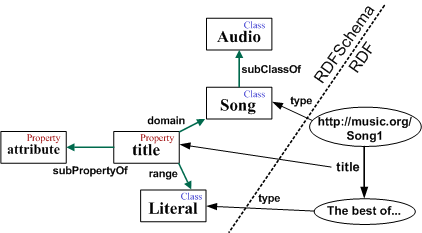
\includegraphics[width=0.8\columnwidth]{images/RDFSchema.png}
	\caption{RDF Schema sample}
	\label{fig:images_rdfs_sample}
\end{figure}

\begin{listing}[H]
  \inputminted[linenos,
               numbersep=5pt,
               breaklines=true,
               frame=lines]{TURTLE}
               {./samples/sample_rdf_schema.ttl}
  \caption{A sample \gls{RDF} data set based on Figure~\ref{fig:images_rdfs_sample}}
\label{lst:sample_rdf_schema}
\end{listing}

As is also shown in Figure~\ref{fig:images_rdfs_sample} the majority of the domain specific knowledge is described in the \gls{RDFS} part of the \gls{RDF} data set. It holds all available classes, predicates, restrictions, \ldots, and is therefore more abstract and expressive. The \gls{RDF} part containing the specific instances might be rather small and concrete, consisting of only existing resources with their real predicates. Usually each of the real entities from the \gls{RDF} part refer to its best matching and most descriptive entity from the \gls{RDFS} part (e.g.\ the entity \url{http://music.org/Song1} in the sample is referring to the \emph{Song} class rather than the \emph{Audio} class). \\

In addition to the classes shown above the \gls{RDF} and \gls{RDFS} specifications contain further useful entities and predicates, such as: \@

\begin{table}[H]
\centering
\begin{tabular}{p{4cm}p{7cm}}
\hline
\textbf{Classes} & \textbf{Description} \\
\hline
rdf:Bag & unordered list of entities \\
\hline
rdf:Seq & ordered list of entities \\
\hline
rdf:Alt & list of alternatives or choices \\
\hline
rdf:Container & superclass of all containers \\
\hline
\textbf{Predicates} & \textbf{Describes} \\
\hline
rdfs:seeAlso &	links to an external resource, that contains additional information \\
\hline
rdfs:isDefinedBy & links to the original definition of a resource \\
\hline
rdfs:Comment & comments and notes on entities \\
\hline
rdfs:Label & human friendly label for entities \\
\hline
\end{tabular}
\caption[\gls{RDF} and \gls{RDFS} supplemental vocabularies]{\gls{RDF} and \gls{RDFS} supplemental vocabularies \citep[pg. 89-90]{antoniou2008semantic}}
\label{tab:w3c_vocab_supplement}
\end{table}

Missing features in RDFS: \ldots  \\
Complex Ontologies in Web Ontology Language (OWL): \ldots \\

% section semantic_ontologies (end)

\subsection{Query Language}
\label{sec:semantic_querylang}

SPARQL requires a \textbf{triple store} - a database containing RDF documents \\
is also referred to as a \textit{Graph Store} \\
data is inserted via Bulk load operation or via SPARQL update statements \\
SPARQL consist of SPARQL Queries that are send over the SPARQL protocol \\
Clients sends the queries to an HTTP endpoint \\
Stores on the public Web incl. dbpedia.org, ckan.org, wikidata.org \\
SPARQL also works with RDFS \\
SPARQL has similarities to SQL:
- each element in a triple might be replaced with a variable like `?varName' like so: \\

\begin{listing}[H]
	\begin{minted}[linenos,
	               numbersep=5pt,
	               gobble=2,
	               frame=lines,
	               framesep=2mm]{SPARQL}
	  PREFIX ns1:<URI>
	  PREFIX ns2:<URI>
	  PREFIX ns3:<URI>

	  SELECT ?varName
	  WHERE {
	      ns1:subject ns2:predicate ?varName
	  }
	\end{minted}
\caption{Selecting information with \gls{SPARQL}}
\label{lst:select_sparql}
\end{listing}

- in the WHERE clause it hosts the graph pattern to match (could be cascaded to go down subgraphs) \\
- variables can occur at any place in the graph pattern (?subj ?pred ?obj) as select with query everything \\
\\
LIMIT \textless n\textgreater option at the end for limiting the result set \\
FILTER (?varName \textless condition\textgreater ) in graph pattern can restrict results to match some
literal values and supports: \\
- numbers, dates: \textless, \textgreater, = \\
- strings: =, regex() \\
\\
\textbf{open world} assumption: resources on the Web are described in different schematas with various properties
using different vocabularies \\
- UNION option in graph pattern combines different matches \\
- OPTIONAL option in graph pattern only returns those entities if they are available (otherwise empty) \\
\\
ASK query checks for the existence of a given graph pattern \\
CONSTRUCT can be used to retrieve a subgraph from a larger graph, can also be used to translate between different schemas \\

\begin{listing}[H]
	\begin{minted}[linenos,
	               numbersep=5pt,
	               gobble=2,
	               frame=lines,
	               framesep=2mm]{SPARQL}
	  PREFIX ns1:<URI>
	  PREFIX ns2:<URI>
	  PREFIX ns3:<URI>

	  CONSTRUCT {
	      ?varA ns2:predicate ?varB .
	      ?varA ns3:predicate ?literalA .
	  }
	  WHERE {
	      ?varA ns1:predicate ?varB
	  }
	  FILTER ( ?varB > x )
	\end{minted}
\caption{A CONSTRUCT query in \gls{SPARQL}}
\label{lst:construct_sparql}
\end{listing}

- SPARQL can be used to harmonize graphs from different sources \\
- is also used for basic reasoning ala ``if found this, assume that'' \\
- can ease hierarchical queries with * or + on the predicate (SPARQL 1.1) \\
- can help resolving issues with different entities referring to the same object (MKP pg. 95)\\
- Federated Queries can be used to combine information from distinct sources via SPARQL (MKP pg. 110-112)\\
\\
- inferencing information from existing triples via SPIN (SPARQL Inferencing Notation) \\
- like in a taxonomy items can be categorized in an hierarchy (MKP pg. 114) \\
- inference patterns are used in Semantic Web applications (MKP pg. 115) \\
   * subClassOf - type propagation rule \\
- inferencing could be done at query time or persistently (MKP pg. 120/121) \\
- inferences can also be helpful when combining information from unknown sources \\
- inferencing happens on various levels (RDFS, RDFS+, OWL) with an increased set of complex inferencing rules (MKP pg. 122/123)
\\
% section semantic_querylang (end)

% section semantic_web (end)
